

\subsubsection{Cadre Général}

Ce module intervient après la phase d'analyse qui lui fourni, par l'intermédiaire de la mémoire, l'environnement courant et un ensemble de formes reconnues. Le \og moteur de choix \fg{} se sert alors de la probabilité d'apparition des annotations associées aux formes reconnues afin d'annoter l'environnement courant.

\subsubsection{Application aux jeux de plateau}

Dans le cadre des jeux de plateau, le moteur de choix reçoit en entrée un ensemble de plateaux avec chacun un ensemble de formes reconnues. Chaque plateau correspond au plateau résultant d'un coup possible. On peut donc dire que le moteur de choix doit choisir entre les différents \og futurs possibles \fg{}. Afin d'évaluer la probabilité de gain d'un plateau, celui-ci fera la moyenne des probabilité de gain des différentes forme reconnues sur ce plateau. Il choisi finalement l'environnement qui maximise la probabilité de gain.

\begin{figure}[H] 
  \begin{center}
		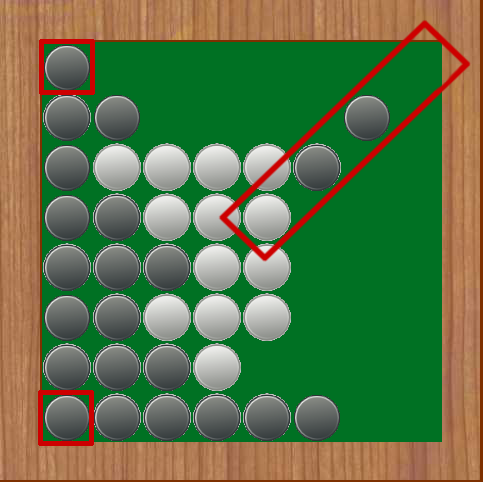
\includegraphics[width=0.3\textwidth]{files/raisonneur/moteur_de_choix} 
	\end{center}
\caption{Représentation graphique de l'environnement} 
\label{img_env}
\end{figure}
